\documentclass[a4paper, USenglish, 11pt]{report}

% Packages
\usepackage{packages/uiomasterfp/uiomasterfp}
\usepackage{graphicx}
\usepackage{titlesec}
\usepackage{cite}
\usepackage{hyperref}
\usepackage{amsmath}
\usepackage{booktabs}
\usepackage{caption}
\usepackage{lscape}
\usepackage{tabularx}
\usepackage{float}
\usepackage{url}
\usepackage{tikz}
\usepackage{minted}
\usepackage{palatino}
\usepackage{microtype}
\usepackage{setspace} 
\usepackage{listings}
\usepackage{tocloft}
\usepackage[USenglish]{babel} 

% Hyperref setup
\hypersetup{
    colorlinks=false, 
    hidelinks
}

% Tikz setup
\usetikzlibrary{shapes.geometric, arrows.meta, positioning, shapes.multipart}

% Minted setup
\usemintedstyle{default}
\setminted[c]{
  frame=lines,
  framesep=2mm,
  baselinestretch=1.2,
  bgcolor=gray!10,
  fontsize=\footnotesize,
  linenos,
  firstnumber=1,
  breaklines,
  autogobble
}

% Custom colors
\definecolor{eth}{HTML}{FAB900}     % BeeGFS
\definecolor{eth2}{HTML}{FFC92E}    % BeeGFS light
\definecolor{dis}{HTML}{389E9B}     % Dolphin
\definecolor{dis2}{HTML}{4ABFBB}    % Dolphin light
\definecolor{ssocks}{HTML}{DD0001}  % UiO
\definecolor{ssocks2}{HTML}{FF1112} % UiO light
\definecolor{sisci}{HTML}{CF24AA}   % Pink
\definecolor{sisci2}{HTML}{DF47BE}  % Pink light
\definecolor{ib}{HTML}{76B900}      % Nvidia
\definecolor{ib2}{HTML}{97EC00}     % Nvidia light

% Misc Setiings
\setlength{\parindent}{0pt}
\setlength{\parskip}{\baselineskip}
\titleformat{\chapter}[hang]{\normalfont\huge\bfseries}{\thechapter}{1em}{}
\setstretch{1.5} 
\bibliographystyle{acm}

% Front page 
\author{Benjamin Borge}
\title{RDMA Integration for BeeGFS over PCIe NTB Interconnects}
\subtitle{Leveraging Dolphin Interconnect Solutions for Parallel Filesystems}

\begin{document}

% Second page
\uiomasterfp[program={Informatics: Programming and System Architecture},color=pink, supervisors={Håkon Kvale Stensland\and Tore Heide Larsen \and Jonas Markussen}]

% Abstract
\begin{abstract}
The abstract should be the last thing to be written. The abstract should be the last thing to be written. The abstract should be the last thing to be written. The abstract should be the last thing to be written. The abstract should be the last thing to be written. The abstract should be the last thing to be written. The abstract should be the last thing to be written. The abstract should be the last thing to be written. The abstract should be the last thing to be written. The abstract should be the last thing to be written. The abstract should be the last thing to be written. The abstract should be the last thing to be written. The abstract should be the last thing to be written. The abstract should be the last thing to be written. The abstract should be the last thing to be written. The abstract should be the last thing to be written. The abstract should be the last thing to be written. The abstract should be the last thing to be written. The abstract should be the last thing to be written. The abstract should be the last thing to be written. 
\end{abstract}

% Roman page numbering
\pagenumbering{roman}
\setcounter{page}{3}

% Acknowledgments
\section*{Acknowledgments}
\newpage

% TOC
\tableofcontents

% Lists
\newpage
\listoffigures
\newpage
\listoftables
\newpage
\listoflistings
\newpage

% Arab page numbering
\pagenumbering{arabic}

% Chapters
\chapter{Introduction}

\section{Motivation}
In an era where scientific discovery and technological innovation are accelerating at unprecedented rates, high-performance computing (HPC) has become the backbone of global advancement. From simulating complex molecular interactions to modeling climate change, HPC systems allow us to address challenges once thought impossible. As data demands grow, even the smallest improvements in these systems can make a difference. Integrating Remote Direct Memory Access (RDMA) with BeeGFS over PCI Express could offer one such subtle push, where every gain—no matter how incremental—helps optimize performance and sustain the momentum of progress.
\section{Problem Statement}


HPC environments require storage solutions that can handle large amounts of data with minimal delay and maximum speed. BeeGFS™, developed by ThinkParQ, is a global shared parallel filesystem widely used in HPC for its scalability and high performance. While BeeGFS can use different network setups with TCP/IP, it relies on RDMA only when connected through InfiniBand networks. RDMA improves data transfer speeds and reduces delays by allowing computers to directly access each other's memory, bypassing the operating system and the CPU.
\\\\
However, when BeeGFS operates over PCI Express (PCIe) Non-Transparent Bridge (NTB) connections provided by Dolphin Interconnect Solutions, it cannot use RDMA and instead relies on standard TCP/IP protocols. This limitation may increase delay and reduce overall performance, impacting data-intensive HPC applications that rely on fast data access and transfers.
\\\\
Dolphin Interconnect Solutions offers SuperSockets, a technology that enables RDMA over PCIe NTB. Integrating SuperSockets into BeeGFS could enable RDMA over PCIe NTB, reducing delay and boosting bandwidth compared to TCP/IP. 
\\\\

The goal of this thesis is to integrate SuperSockets™ into BeeGFS to enable RDMA over Dolphin’s PCIe NTB Fabric. This integration aims to reduce latency and increase bandwidth, improving BeeGFS performance in HPC environments that use PCIe NTB networks. The work will involve modifying the BeeGFS source code to support SuperSockets and conducting a performance evaluation. This evaluation will compare BeeGFS with RDMA over PCIe NTB against the existing RDMA setup over InfiniBand and the current PCIe setup over TCP/IP. Key metrics for comparison will include latency, bandwidth, and overall system performance.

\section{Research Objectives}
The main objective of this thesis is to integrate PCIe RDMA functionality into BeeGFS. This integration will use PCIe NTBs from Dolphin Interconnect Solutions to reduce latency, increase bandwidth, and improve reliability in HPC environments.

\subsection{Specific Objectives}
\begin{itemize}
    \item \textbf{Integration of SuperSockets into BeeGFS}: Modify the BeeGFS codebase to support SuperSockets, enabling RDMA over PCIe NTB networks.
    \item \textbf{Performance Evaluation}: Assess the impact of SuperSockets integration on BeeGFS performance metrics such as latency, bandwidth, and throughput.
    \item \textbf{Comparative Analysis}: Compare the performance of BeeGFS over PCIe NTB with SuperSockets against its performance over InfiniBand networks with existing RDMA support.
    \item \textbf{Feasibility Study}: Analyze the practicality and benefits of extending RDMA support in BeeGFS to PCIe NTB networks for broader applicability in HPC infrastructures.
\end{itemize}

\subsection{Research Questions}
\begin{enumerate}
    \item \textit{How can SuperSockets be effectively integrated into the BeeGFS filesystem to enable RDMA over PCIe NTB networks?}
    \item \textit{What are the performance improvements in terms of latency and bandwidth when using BeeGFS with SuperSockets over PCIe NTB compared to standard TCP/IP communication?}
    \item \textit{How does the performance of BeeGFS with SuperSockets over PCIe NTB compare to its performance with RDMA over InfiniBand networks?}
    \item \textit{What challenges may arise during the integration of SuperSockets into BeeGFS, and how can they be addressed?}

\end{enumerate}

\section{Scope and Limitations}
\subsection{Scope}
This thesis focuses on the technical integration and performance evaluation of SuperSockets within the BeeGFS filesystem over PCIe NTB networks. The study encompasses:
\begin{itemize}
    \item \textbf{Software Development}: Modifying the BeeGFS codebase to incorporate SuperSockets support.
    \item \textbf{Experimental Setup}: Configuring an HPC environment/POC using Dolphin's PCIe NTB interconnects for testing and benchmarking.
    \item \textbf{Performance Metrics}: Measuring and analyzing key performance indicators such as latency, bandwidth, and system throughput.
    \item \textbf{Comparative Analysis}: Evaluating the enhanced BeeGFS over PCIe NTB against its existing RDMA implementation over InfiniBand networks.
.
\end{itemize}

\subsection{Limitations}

\begin{itemize}
    \item \textbf{Hardware Constraints}: The experimental results are limited to the specific hardware and network configurations available during the study, which may not represent all possible HPC environments.
    \item \textbf{Generality of Findings}: While the findings aim to be indicative, they may not be directly generalizable to all versions of BeeGFS or different RDMA technologies.
    \item \textbf{Time Constraints}: The scope of the thesis is confined to the allocated time frame, which may limit the depth of exploration into advanced optimizations or extended testing scenarios.
    \item \textbf{Focus on SuperSockets (?)}: The study specifically investigates SuperSockets integration and does not explore alternative methods of enabling RDMA over PCIe NTB networks. ! May use SISCI here..
    \item \textbf{Software Stability}: Potential stability issues arising from modifications to the BeeGFS codebase may affect performance results and require additional troubleshooting beyond the thesis scope.
\end{itemize}

\chapter{Background}

% TODO: Refine, write about importance
\section{History of HPC}
High-performance computing has a long history of driving advancements in science and technology. It began in the mid-20th century with the development of early computing systems such as the ENIAC in 1945, which was designed to handle complex calculations that were previously impossible. However, it was the introduction of the CDC 6600 in 1964, designed by Seymour Cray, that is widely regarded as the birth of modern supercomputing.\cite{cook2015history} This machine introduced parallel processing and vector computation, both key concepts that have shaped the evolution of HPC. 
\\\\
Throughout the 1970s and 1980s, supercomputing continued to advance, with systems like the Cray-1 in 1976 bringing higher processing speeds and improved efficiency through vector processing. These developments were crucial for fields such as physics, weather forecasting, and large-scale simulations, which required enormous amounts of computational power. The 1990s saw further innovation with the rise of massively parallel processing (MPP) systems, which used thousands of processors to perform calculations simultaneously. During this time, the Beowulf cluster architecture also emerged, enabling more affordable and scalable supercomputing by using standard hardware components.
\\\\
In the 21st century, HPC has continued to grow in importance, with systems reaching petascale performance, such as IBM’s Roadrunner in 2008, which was capable of over one quadrillion calculations per second (1 petaflop). Today, the field is moving towards exascale computing, with new systems like Frontier aiming to exceed one exaflop ($10^{18}$ floating-point operations per second).\cite{top500_2024} These advancements enable increasingly complex scientific research, including large-scale data analysis, climate modeling, and artificial intelligence.
\\\\
As HPC systems evolve, improving individual components becomes essential to meet rising computational demands. Technologies like RDMA offer significant performance gains by enabling direct memory access between systems, reducing CPU involvement and improving data transfer speeds. 

\section{IO as a bottleneck}
In HPC clusters, I/O performance is critical to ensure that applications can efficiently read and write large volumes of data. However, I/O often becomes a significant bottleneck, limiting the overall performance of applications.\cite{9355272}
\\\\
A main cause of I/O bottlenecks in HPC clusters is the centralized or sequential data access patterns common in traditional filesystems, which are not built to support multiple processes accessing data at the same time. In HPC clusters, thousands of compute nodes may try to read or write data simultaneously, which can overwhelm standard storage systems and create I/O contention. This problem is especially noticeable in data-intensive workloads, where frequent access to large datasets intensifies contention and reduces effective I/O throughput.
\\\\
To overcome these limitations, parallel filesystems are essential in HPC storage systems. Parallel filesystems like BeeGFS, Lustre, and GPFS (! is parallel?) are designed to spread data across multiple storage nodes, allowing many processes to access data at the same time. By managing data in parallel, these filesystems can handle high I/O demands and reduce contention, avoiding the bottlenecks common in traditional storage systems. Parallel filesystems use striping of data across multiple storage nodes, allowing data to be read and written at the same time across these nodes. This setup improves data access speeds and reduces bottlenecks, as the workload is shared rather than focused on one location.

\section{BeeGFS}
BeeGFS (before: Fraunhofer Parallel File System) is a high-performance, parallel file system designed for use in HPC clusters. Originally developed by the Fraunhofer Institute for Industrial Mathematics, BeeGFS is engineered to scale out horizontally across multiple servers, distributing file data and metadata across multiple nodes. This architecture allows BeeGFS to handle intensive workloads by spreading I/O operations over multiple storage nodes, enhancing both performance and data redundancy. It supports both traditional storage setups and modern architectures, such as NVMe and SSDs, which makes it adaptable for various HPC configurations.
\\\\
One of the key features of BeeGFS is the ability to separate metadata from file data, enabling efficient handling of file system operations like lookups, renames, and access permissions. There are designated meta data nodes. This division means that metadata operations don’t interfere with data transfer, resulting in faster file operations and improved overall system performance. BeeGFS also includes other features, like monitoring, quotas/groups and data mirroring. Additionally, BeeGFS integrates easily with existing infrastructure and supports standard POSIX file system rules.

\section{Remote Direct Memory Access}
Remote Direct Memory Access (RDMA) is a technology that enables high-speed data transfer between memory spaces on different systems without involving the CPU, operating system, or I/O buffers. This bypass of traditional networking layers allows for extremely low-latency communication and high throughput, which is  beneficial in HPC where efficient data movement is critical. RDMA operates by allowing one system to read or write directly into the memory of another over a network, typically via standards like InfiniBand or RDMA over Converged Ethernet (RoCE).
\\\\
When establishing an RDMA connection, specific memory regions need to be registered with the NICs to allow direct data access. This memory registration step assigns certain memory areas to the NICs, giving permission to access these addresses directly.
\\\\
After memory registration, RDMA establishes a queue pair (QP) connection, which includes a send queue and a receive queue. Each side of the connection places work requests (like read, write, or send) into these queues. The NIC then handles these requests independently, without needing the CPU to get involved. 


\section{PCI Express}
PCI Express (PCIe) is a high-speed interface standard for connecting various hardware components within a computer, such as CPUs, GPUs, storage devices, and network interfaces. It uses a point-to-point architecture, where each device has its own direct connection to the chipset. This setup reduces data congestion and allows for much faster data transfers compared to older, shared-bus designs.
\\\\
PCIe connections are made up of lane—pairs of paths for sending and receiving data. Devices can use multiple lanes (like x4, x8, or x16) to increase bandwidth according to their needs. Each new generation of PCIe has doubled the transfer speed per lane, supporting high-performance devices such as GPUs and NVMe storage with the bandwidth they require.
\\\\
Although PCIe is mainly used for connecting components within a single computer, it can also link the memory of two separate computers, allowing for direct, high-speed data transfer between them.


\section{Dolphin Interconnects}
Dolphin Interconnect Solutions develops high-performance networking products that use RDMA and PCI Express to achieve extremely low-latency data transfer between computing nodes. By combining RDMA’s direct memory access with PCIe’s high-speed architecture, Dolphin enables data to move directly between devices without needing CPU intervention. Using PCIe as the foundation, Dolphin interconnects allow peer-to-peer communication between nodes, bypassing traditional network layers to reduce latency and increase data transfer speeds, which improves efficiency for data-intensive tasks.

\subsection{SuperSockets}
SuperSockets is Dolphin’s high-performance socket API extension designed to offer an easy extension for applications that rely on traditional TCP/IP sockets. SuperSockets enable faster speeds while still using familiar socket interfaces since the data is transfered using RDMA. By bypassing much of the operating system overhead associated with traditional network stacks, SuperSockets facilitate direct, high-speed communication between nodes with minimal latency, taking advantage of RDMA and PCIe capabilities. This results in  performance improvements for distributed applications and is  beneficial for data-intensive workloads in HPC.

\subsection{SISCI}
SISCI (Software Infrastructure for Shared-Memory Cluster Interconnect) provides an API for applications needing direct memory access and memory sharing across multiple nodes. SISCI supports high-level abstractions for memory allocation, mapping, and synchronization. By leveraging PCIe’s peer-to-peer capabilities, SISCI enables processes on different nodes to access and manipulate each other's memory regions without CPU involvement, reducing latency and increasing throughput. SISCI also have PIO support.

\subsection{Dolphin IPoPCIe}
Dolphin’s IPoPCIe driver provides a transparent way to send and receive network traffic over PCI Express instead of Ethernet. By combining Programmed I/O (PIO) with RDMA transfers, it reduces system overhead and achieves significantly higher bandwidth and lower latency than standard Ethernet solutions. IPoPCIe still presents a TCP/IP interface to the operating system and applications. . However, IPoPCIe typically reduces latency by a factor of 5–6 compared to 10G Ethernet, while also delivering much higher data throughput, often over 50 Gbps in a standard x8 Gen3 PCIe configuration without requiring changes to user application. \cite{dolphin_fast_tcp_udp_ip}
\chapter{System Design and Implementation}

This chapter outlines the technical design choices and the integration of SuperSockets into the BeeGFS codebase. It begins with a design overview and a review of the existing logic in the source code, followed by implementation details and validation. Finally is a summary of the scripting logic used in the work.

\section{Design Overview}

SuperSockets are designed for plug-and-play integration, requiring minimal changes to existing systems. The implementation follows the standard socket logic flow to ensure compatibility.

The client kernel module operates in kernel space, so kernel-space SuperSockets must be used. For other components, both userspace and kernel-space implementations are provided.

In the userspace implementation, application code remains unmodified. Interception of socket calls is achieved using \texttt{LD\_PRELOAD}.

\section{Existing Logic}

BeeGFS has, as described in the background chapter, multiple services or components. The BeeGFS source tree is structured by service, with every component residing in a separate directory and building independently. It also includes a \texttt{common} directory that holds shared code used across components. While most of the codebase is written in C++, the client kernel module is implemented in C. Socket logic is shared mainly between components.

Sockets play a central role in BeeGFS, enabling clients to connect to metadata servers to locate files and to storage servers to read or write file chunks. Metadata and storage servers also communicate with each other to ensure data consistency.
BeeGFS uses TCP for reliable, stream-based file transfers and UDP for less critical messages like heartbeat messages to the management service. To support many simultaneous connections, BeeGFS uses connection pooling, which reduces the overhead of creating new connections for frequent operations like metadata updates or data streaming.

The system selects the best network interface for each connection, whether Ethernet or InfiniBand.

BeeGFS abstracts low-level socket operations through a layered class structure. At the core is the \texttt{Socket} class, which handles basic network actions like connecting, binding, and formatting addresses. Building on this, the \texttt{PooledSocket} class supports connection pooling, timeouts, and connection reuse—key for managing resources efficiently in large-scale environments.

The \texttt{StandardSocket} class extends this further by implementing full socket behavior, including \texttt{epoll}-based non-blocking I/O, configuration of socket options, and support for both TCP and UDP. These sockets are used for data transfers, metadata queries, and internal communication between BeeGFS components.

BeeGFS also scans available network interfaces using the \texttt{NetworkInterfaceCard} class to support high-performance networking. It discovers standard TCP/IP interfaces and checks for RDMA-capable devices by attempting to bind RDMA sockets to each address. This allows BeeGFS to dynamically choose between standard and high-speed interfaces like InfiniBand, based on availability and configuration.

This modular socket and interface design enables BeeGFS to maintain flexibility, performance, and scalability across different environments and workloads.

BeeGFS uses a \texttt{NodeConnPool} class to manage connections efficiently. Each node maintains a pool of reusable socket connections to other nodes. These are based on the \texttt{PooledSocket} class, which extends basic socket functionality with features like expiration timers, connection reuse, and availability tracking. When a service needs to communicate, it requests a stream socket from the pool, either by reusing an existing connection or establishing a new one.

\texttt{NodeConnPool} automatically selects the best available network interface, supports RDMA and TCP, and applies socket options to optimize performance. It also handles authentication, connection fallback, and clean-up idle or failed sockets. This pooling mechanism reduces overhead, increases scalability, and ensures robust, low-latency communication across the cluster.

\section{Implementation Details}

SuperSockets are designed to be plug-and-play, requiring minimal modifications to the existing networking logic in BeeGFS. The core implementation task involved locating where TCP sockets are defined in the source code and replacing the standard \texttt{AF\_INET} address family with \texttt{AF\_SSOCKS}. This change allows the system to establish socket connections over Dolphin's PCIe-based interconnect rather than through traditional Ethernet. In Listing~\ref{lst:ssocks_construct}, the SuperSocket address family constant is used in the function that creates a standard socket. This implementation resides in \texttt{StandardSocket.c}. The function is called from \texttt{NodeConnPool.c}, where client-side socket management is handled. A similar structure is used in the C++ implementation for the user-space daemons. The full source code is available in the linked GitHub repository.

In the current implementation, the \texttt{AF\_SSOCKS} constant is hardcoded into the codebase. A more robust approach would involve dynamically retrieving the assigned address family value at runtime, which is discussed further in the future work section.

By default, SuperSockets use address family 27. However, this conflicts with \texttt{AF\_SDP\_INET}, which is associated with the Socket Direct Protocol (SDP) used in InfiniBand environments~\cite{goldenberg}. To avoid this conflict, the address family was explicitly set to 34 using Dolphin's configuration mechanism. This value was specified in the \texttt{dis\_ssocks.conf} file.

UDP sockets in the BeeGFS codebase were left unchanged. These sockets are used solely for lightweight heartbeat messages and do not contribute to the performance of data transfer operations. As such, they continue to operate over standard Ethernet interfaces.
 
\begin{listing}[H]
\begin{minted}[label={lst:ssocks_construct}]{c}
StandardSocket* StandardSocket_constructUDP(void) {
   return StandardSocket_construct(PF_INET, SOCK_DGRAM, 0);
}

StandardSocket* StandardSocket_constructTCP(void) {
   return StandardSocket_construct(PF_SSOCKS, SOCK_STREAM, 0);
}

StandardSocket* StandardSocket_constructSDP(void) {
   return StandardSocket_construct(PF_SDP, SOCK_STREAM, 0);
}
\end{minted}
\caption{Kernel Module Socket Construction}
\end{listing}

The \texttt{AF\_SSOCKS} address family is also defined in the \texttt{NetworkInterfaceCard} class. This class is responsible for detecting and managing network interfaces, and for distinguishing between TCP and existing RDMA functionality. It opens a new socket to interact with the network stack.

\section{Validation}

Dolphin Interconnect Solutions provides a utility called \texttt{dis\_ssocks\_stat}, which displays real-time information about active SuperSockets connections on a system. Since SuperSockets automatically falls back to TCP/IP if a connection fails, this tool helps determine whether data is transmitted via SuperSockets or the fallback method. Specifically, it reports the number of bytes sent and received through SuperSockets and fallback TCP/IP. Listing \ref{lst:ssocks_stat} shows an example of terminal output from \texttt{dis\_ssocks\_stat} during a successful SuperSockets file transfer in BeeGFS.

\begin{listing}[H]
\begin{minted}[
  linenos        = false,
  style          = vs,
  bgcolor        = gray!10,
  fontsize       = \small,
  highlightlines = {1},            % which line(s) to colour
  highlightcolor = purple!20,
]{cucumber}
./dis_ssocks_stat -G
STREAM: 20
DGRAM: 0 (1 tx, 1 rx)
RDS: 0
SuperSockets in: 185112645 (176 MiB)
SuperSockets out: 17095 (0 MiB)
Fallback in: 0 (0 MiB)
Fallback out: 0 (0 MiB)
TX:  0.0% poll,  0.0% block
RX:  0.0% poll,  0.0% block
Interrupts TX: 370 req, 357 noreq, 0 task
Interrupts RX: 0 req, 6094 noreq, 0 task
Inline: 0 crc, 0 resend, 0 discard
\end{minted}
\caption{Terminal output of SuperSockets statistics}
\label{lst:ssocks_stat}
\end{listing}

\section{Scripts}

Several scripts were developed throughout this work to facilitate various tasks related to software development, performance testing, and data analysis. These scripts, available in the attached repository, automated repetitive processes, reduced manual effort, and ensured consistency across different stages of experimentation.

The \texttt{cp-binaries} script automates the transfer of compiled binary files to their designated directories. Streamlining this process ensures that the most recent versions of binaries are consistently available for testing, minimizing the potential for errors caused by manual copying.

The \texttt{fio-run} script manages the execution of performance benchmarks using the Flexible I/O Tester (FIO). It simplifies and standardizes the benchmarking process, facilitating consistent, reproducible evaluations of storage performance under various configurations and workloads.

The \texttt{enable-if} script simplifies the enabling and disabling of network interfaces. This functionality is useful when switching between interfaces during benchmarking. It works by manipulating the \texttt{connInterfacesFile}.

The \texttt{beegfs-swap} script facilitates convenient switching between different BeeGFS builds, streamlining debugging, testing, and benchmarking workflows. It provides options to swap individual BeeGFS services or all services simultaneously. Additionally, the script supports comparing the currently deployed build with the version under development.

The \texttt{beegfs-service} script provides capabilities for managing BeeGFS services. Since BeeGFS services must be initiated and terminated in a specific sequence, this script ensures the correct ordering. Additionally, it saves time by allowing all services to be started or stopped simultaneously.

The \texttt{sync} script handles synchronization of files between computers with the help of \texttt{rsync}.

The \texttt{div} script supports dividing large datasets or log files into smaller, manageable segments. This capability is particularly beneficial for parallel processing, detailed analysis, and iterative testing processes.

The series of \texttt{make\_img\_*} scripts serve as configuration tools for the Matplotlib-based Python plotting scripts. They are designed to generate multiple plots efficiently, with the flexibility to adjust plot settings for individual plots easily.

\chapter{Results}

\section{Testbed Configuration}

\subsection{Minimal Testbed}

To begin testing, a testbed consisting of two similar computers was set up. These two nodes, served as both storage servers and metadata servers. This setup is relatively simple compared to large HPC clusters, which typically have dedicated storage and metadata nodes. Both nodes are identical in terms of hardware and software specifications.

\subsubsection{Hardware Specifications}
\begin{table}[H]
    \centering
    \caption{Hardware Specifications}
    \label{tab:node_specs}
    \begin{tabularx}{\textwidth}{|X|X|}
        \hline
        \textbf{Model} & MSI Z97-G55 \\
        \hline
        \textbf{CPU Model} & Intel Core i5-4590 @ 3.30GHz x 4 \\
        \hline
        \textbf{Memory} & 2 x 4GB DDR3 @ 1600MHz \\
        \hline
        \textbf{Storage} & 4 TB HDD - 250 GB SSD\\
        \hline
        \textbf{PCIe Version} & 3.0 \\
        \hline
        \textbf{PCIe Lanes} & - \\
        \hline
        \textbf{PCIe NTB} & - \\
        \hline
        \textbf{HDD Interface} & SATA 6 Gb/s \\
        \hline
        \textbf{HDD Cache} & 64MB \\
        \hline
        \textbf{HDD Throughput Max} & 180 MB/S \\
        \hline
        \textbf{HDD Average Data Rate} & 146 MB/S \\
        \hline
        \textbf{HDD Avarage Latency} & 5.16 ms \\
        \hline
    \end{tabularx}
\end{table}

\subsubsection{Software Specifications}
\begin{table}[H]
    \centering
    \caption{Software Specifications}
    \label{tab:software_specs}
    \begin{tabularx}{\textwidth}{|X|X|}
        \hline

        \textbf{Operating System} & Ubuntu 22.04.5 \\
        \hline
        \textbf{Kernel Version} & 6.8.0-52-generic \\
        \hline
        \textbf{BeeGFS Version} & 7.4.5\\ % Fill in
        \hline
        \textbf{eXpressWare Version} & x.x.x \\
        \hline
    \end{tabularx}
\end{table}

\subsubsection{Storage Configuration}
\begin{table}[H]
    \centering
    \caption{Storage Configuration}
    \label{tab:storage_specs}
    \begin{tabularx}{\textwidth}{|l|X|X|X|}
        \hline
        \textbf{Device} & \textbf{Type} & \textbf{Size} & \textbf{Purpose} \\
        \hline
        sda1 & Partition & 37.3 GB (ext4) & Unused \\
        sda2 & Partition & 149 GB (ext4) & BeeGFS metadata \\
        sda3 & Partition & 3.5 TB (XFS) & BeeGFS data \\
        nvme0n1 & NVMe SSD & 232.9 GB (ext4) & OS \\
        \hline
    \end{tabularx}
\end{table}

\subsection{Scaled Testbed}

\subsubsection{Hardware Specifications}

\begin{table}[H]
    \centering
    \caption{Hardware Specifications}
    \label{tab:node_specs}
    \begin{tabularx}{\textwidth}{|X|X|}
        \hline
        \textbf{Model} &  \\
        \hline
        \textbf{CPU Model} &  \\
        \hline
        \textbf{Memory} &  \\
        \hline
        \textbf{Storage} & \\
        \hline
        \textbf{PCIe Version} &  \\
        \hline
        \textbf{PCIe Lanes} &  \\
        \hline
        \textbf{PCIe NTB} & \\
        \hline
        \textbf{SSD Interface} & \\
        \hline
        \textbf{SSD Cache} &  \\
        \hline
        \textbf{SSD Throughput Max} &  \\
        \hline
        \textbf{SSD Average Data Rate} &  \\
        \hline
        \textbf{SSD Avarage Latency} & \\
        \hline
    \end{tabularx}
\end{table}

\subsubsection{Software Specifications}

\begin{table}[H]
    \centering
    \caption{Software Specifications}
    \label{tab:software_specs}
    \begin{tabularx}{\textwidth}{|X|X|}
        \hline

        \textbf{Operating System} &  \\
        \hline
        \textbf{Kernel Version} &  \\
        \hline
        \textbf{BeeGFS Version} & \\ % Fill in
        \hline
        \textbf{eXpressWare Version} &  \\
        \hline
    \end{tabularx}
\end{table}

\subsubsection{Storage Configuration}

\section{Minimal Testbed Results}

\subsection{Throughput vs. Block Size}

Initial performance testing was conducted using two nodes equipped with traditional hard disk drives (HDDs). FIO was used to measure sequential and random read/write performance across various block sizes. In this setup, there were two BeeGFS storage servers, each backed by an HDD with a theoretical maximum throughput of 180 MB/s and an average data rate of 146 MB/s, resulting in an expected combined average of approximately 292 MB/s.

For both sequential reads and writes, IPoPCIe and SuperSockets reached a throughput ceiling of around 260 MB/s, while Ethernet peaked just above 150 MB/s. Output from the \path{sar} tool showed that both disks were operating at 99.7\% utilization, indicating that the throughput bottleneck lies at the disk level.

Sequential read and write operations performed better than random access, which is expected for HDDs. This is because random access requires the disk to move its read/write head to different locations, which takes more time. In contrast, sequential access reads or writes data in order, allowing the disk to work more efficiently.

\begin{figure}[H]
    \centering
    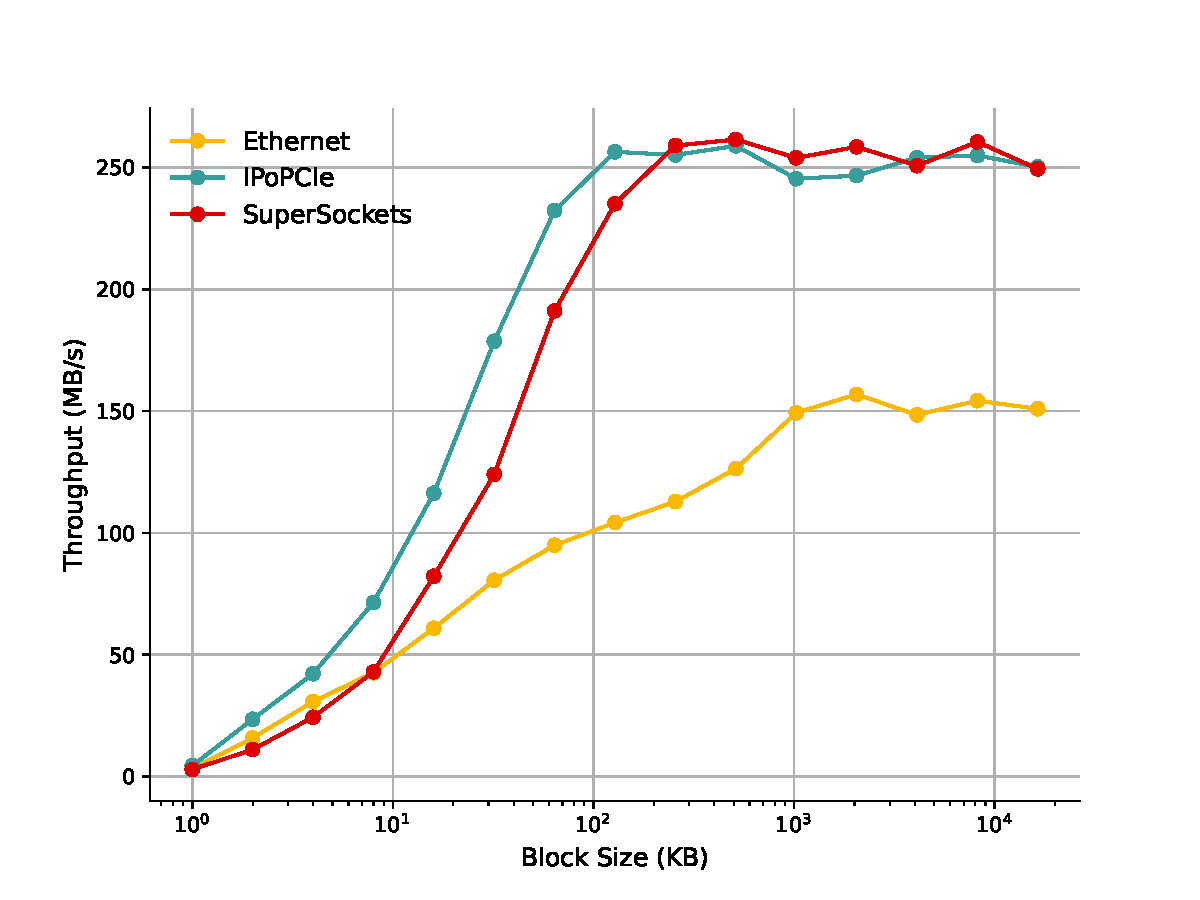
\includegraphics[width=0.99\textwidth]{fig/img/fio/throughput_vs_bs_write_seq_ssocks.pdf}
    \caption{HDD - Throughput vs. Block Size (Sequential Write)}
    \label{fig:hdd_tp_bs_seqread}
\end{figure}
\begin{figure}[H]
    \centering
    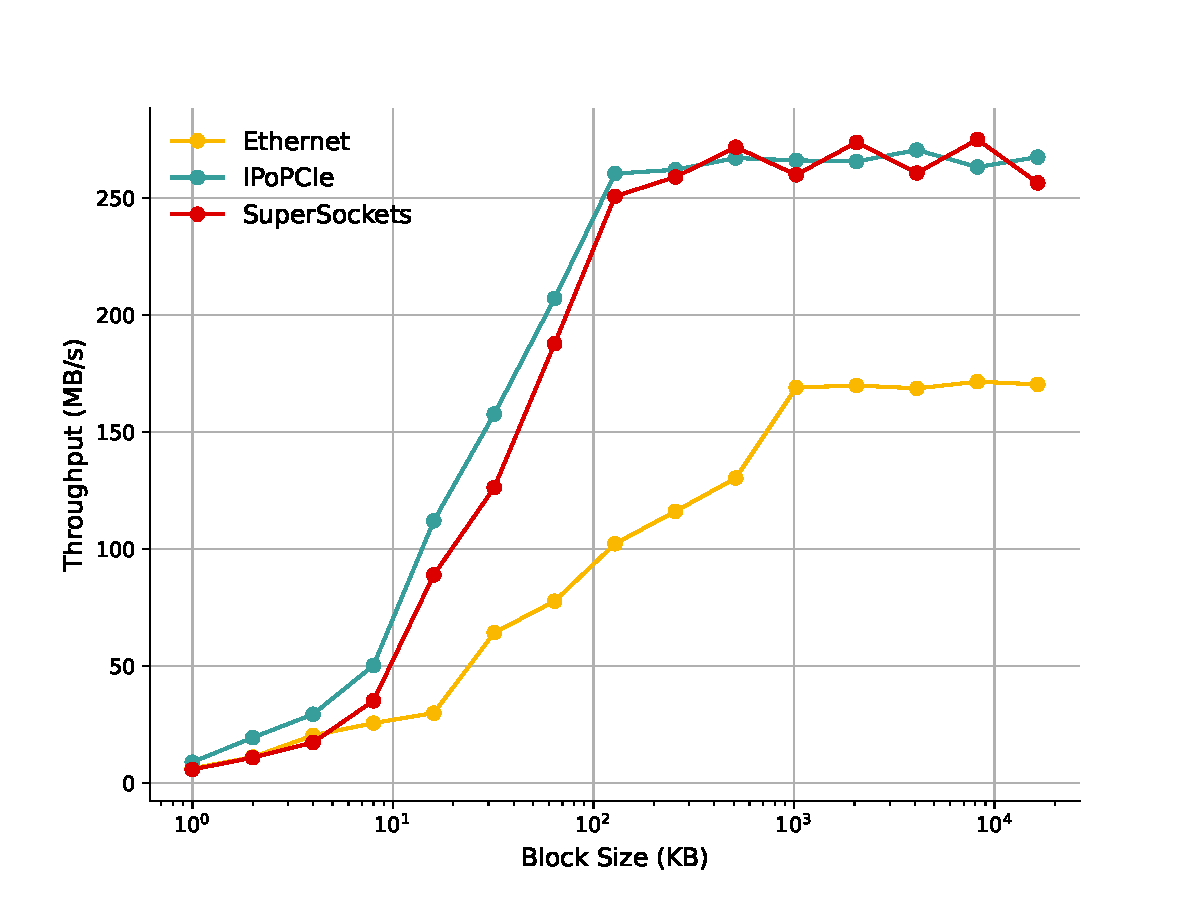
\includegraphics[width=0.99\textwidth]{fig/img/fio/throughput_vs_bs_read_seq_ssocks.pdf}
    \caption{HDD - Throughput vs. Block Size (Sequential Read)}
    \label{fig:hdd_tp_bs_seqread}
\end{figure}

\begin{figure}[H]
    \centering
    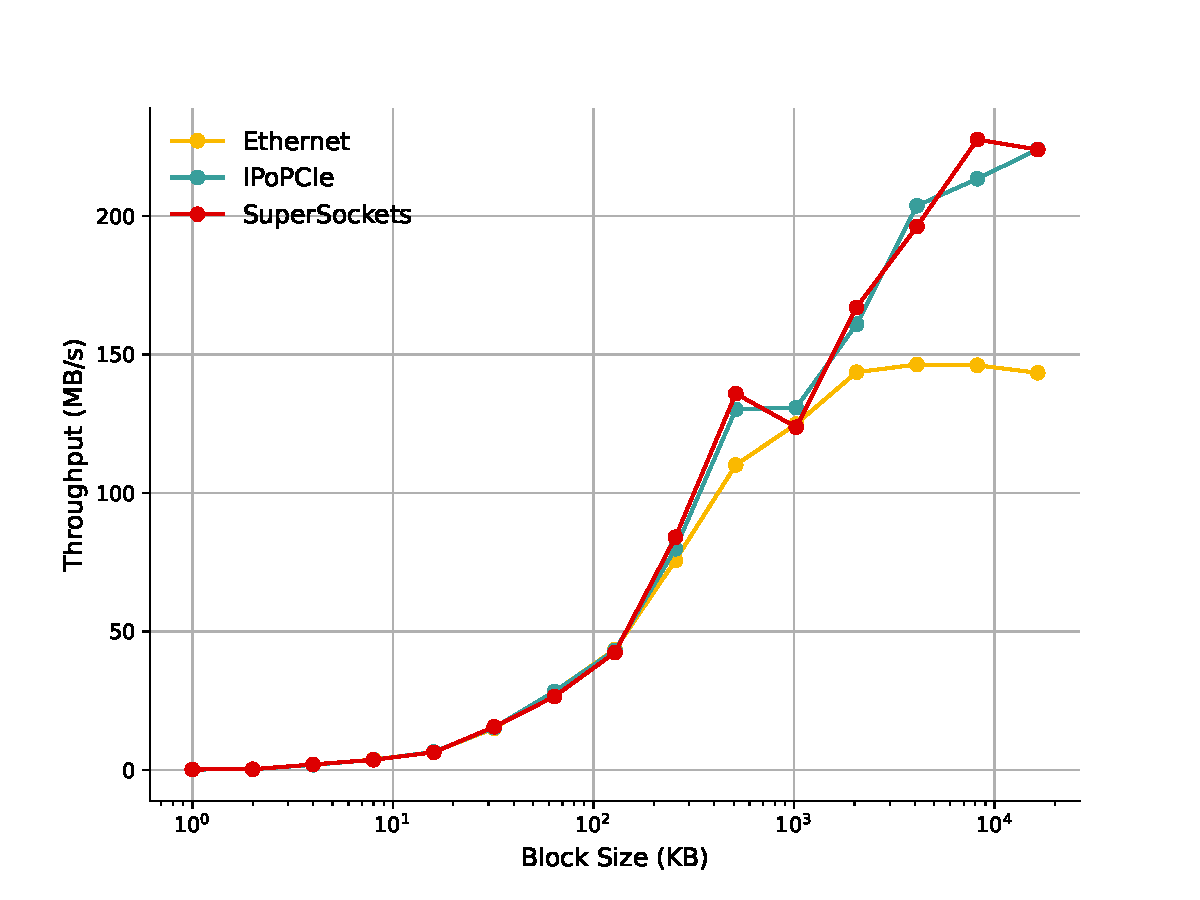
\includegraphics[width=0.99\textwidth]{fig/img/fio/throughput_vs_bs_write_rand_ssocks.pdf}
    \caption{HDD - Throughput vs. Block Size (Random Write)}
    \label{fig:hdd_tp_bs_seqread}
\end{figure}

\begin{figure}[H]
    \centering
    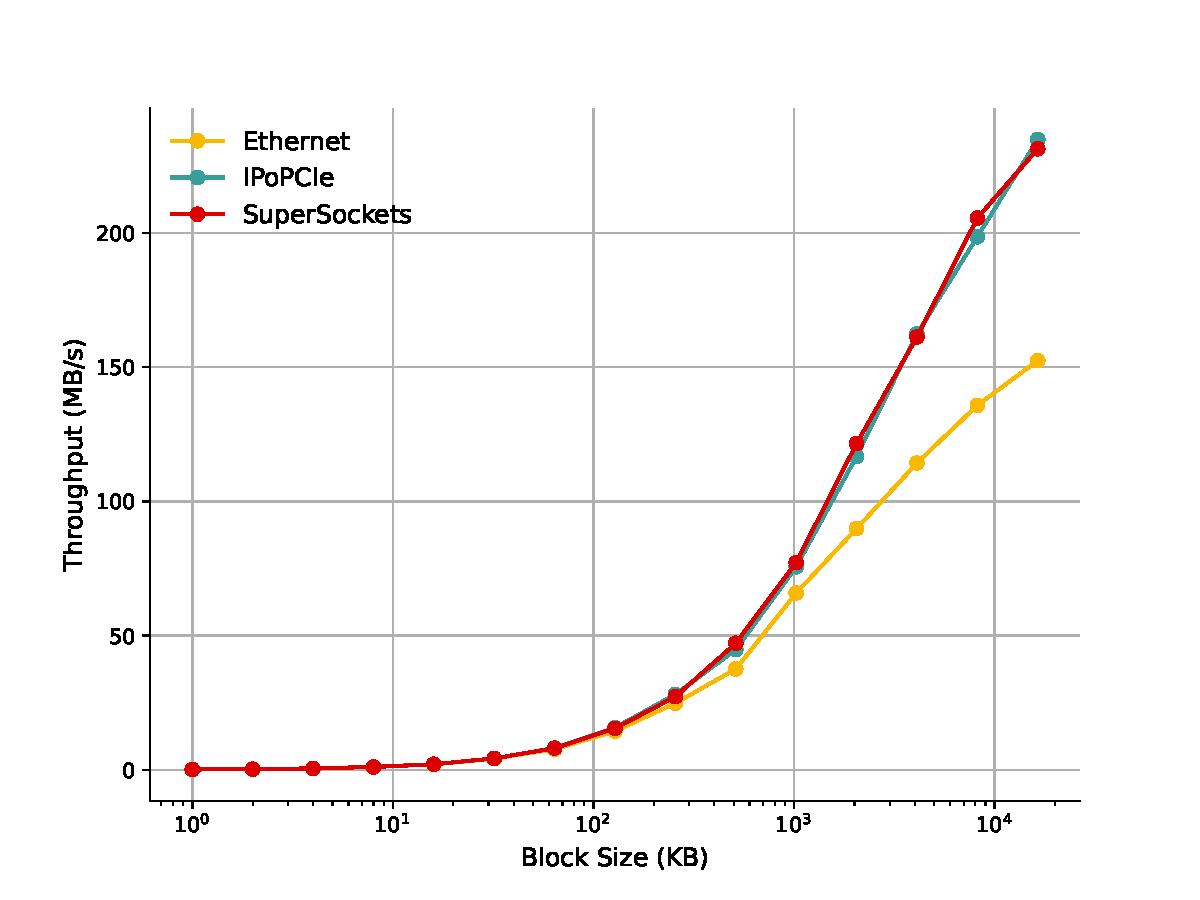
\includegraphics[width=0.99\textwidth]{fig/img/fio/throughput_vs_bs_read_rand_ssocks.pdf}
    \caption{HDD - Throughput vs. Block Size (Random Read)}
    \label{fig:hdd_tp_bs_seqread}
\end{figure}

\section{Scaled Testbed Results}

Currently empty.
\chapter{Discussion}

\section{Interface Comparison}

\section{Hardware Influence}

\section{Key Findings}

\chapter{Conclusion and Future Work}

% References section
\setstretch{1} 
\cleardoublepage
\phantomsection
\addcontentsline{toc}{chapter}{\:\:\:\:\, Bibliography}
\bibliography{references}

% Appendicies
\setstretch{1.25}
\appendix
\chapter{Thesis Repository}
As part of this thesis, a dedicated repository has been created to store all source code, scripts, benchmarking results and other related files. The repository is publicly available at:

\begin{center}
\textbf{\url{https://github.com/multiib/beegfs-thesis}}
\end{center}

This repository includes the following components:

\begin{itemize}
    \item \textbf{Benchmarking Code:} Scripts used to measure throughput, latency, and other performance metrics for IPoPCIe, SuperSockets, and Ethernet.
    \item \textbf{Graph Plotting Scripts:} Python and LaTeX scripts for generating visual representations of benchmarking results.
    \item \textbf{Experimental Results:} Raw data collected from various test runs, formatted for reproducibility.
    \item \textbf{BeeGFS Modifications:} Any relevant code changes made to enable SuperSockets or adjust transport mechanisms.
\end{itemize}

This repository serves as a supplementary resource for this thesis, ensuring that all experiments can be replicated, validated, and extended in future research.


\chapter{Test Outputs}

benjabor@mpg-2014-18:~$ sudo dd if=/dev/random of=/global/D1/testfile-10GB bs=1M count=10240
[sudo] password for benjabor: 
10240+0 records in
10240+0 records out
10737418240 bytes (11 GB, 10 GiB) copied, 34.7378 s, 309 MB/s

\end{document}
